\documentclass[10pt]{article}
\usepackage[letterpaper, margin=1in]{geometry}
\usepackage[T1]{fontenc}
\usepackage{microtype}
\usepackage{amsmath,amssymb}
\usepackage{graphicx}
\usepackage{booktabs}
\usepackage{xcolor}
\usepackage[numbers]{natbib}
\usepackage{floatrow}
\floatsetup[table]{capposition=top}
\floatsetup[figure]{capposition=bottom}
\usepackage[labelsep=colon]{caption}
\usepackage{url}
\definecolor{linkblue}{rgb}{0.0, 0.33, 0.71}
\usepackage[colorlinks=true, citecolor=linkblue, linkcolor=linkblue, urlcolor=linkblue]{hyperref}
\usepackage[capitalize,noabbrev]{cleveref}

% Generated by robust/report.py. Do not edit by hand.
\newcommand{\mAcresM}{7.1}
\newcommand{\mBandsClip}{1.0}
\newcommand{\mBandsFoldFourAfter}{0.686}
\newcommand{\mBandsFoldFourBefore}{0.034}
\newcommand{\mBestUnet}{U-Net, 12 bands + indices}
\newcommand{\mBestUnetMiou}{0.686}
\newcommand{\mCampGenericPhys}{70.5}
\newcommand{\mCampMtbsHigh}{10}
\newcommand{\mCampOrigAgree}{26.1}
\newcommand{\mCampOrigHigh}{53}
\newcommand{\mCampOrigModAsHigh}{87}
\newcommand{\mCampOrigScenes}{43.5}
\newcommand{\mCampStretch}{52.1}
\newcommand{\mDiffBandsLearned}{\ensuremath{-0.001}}
\newcommand{\mDiffBandsLearnedHi}{\ensuremath{+0.012}}
\newcommand{\mDiffBandsLearnedLo}{\ensuremath{-0.013}}
\newcommand{\mDiffGbm}{\ensuremath{+0.008}}
\newcommand{\mDiffGbmHi}{\ensuremath{+0.016}}
\newcommand{\mDiffGbmLo}{\ensuremath{+0.001}}
\newcommand{\mDiffGeneric}{\ensuremath{+0.123}}
\newcommand{\mDiffGenericHi}{\ensuremath{+0.150}}
\newcommand{\mDiffGenericLo}{\ensuremath{+0.096}}
\newcommand{\mDiffIdxBands}{\ensuremath{+0.003}}
\newcommand{\mDiffIdxBandsHi}{\ensuremath{+0.008}}
\newcommand{\mDiffIdxBandsLo}{\ensuremath{-0.004}}
\newcommand{\mDiffLearnGen}{\ensuremath{+0.121}}
\newcommand{\mDiffLearnGenHi}{\ensuremath{+0.146}}
\newcommand{\mDiffLearnGenLo}{\ensuremath{+0.094}}
\newcommand{\mDiffLearned}{\ensuremath{+0.002}}
\newcommand{\mDiffLearnedHi}{\ensuremath{+0.014}}
\newcommand{\mDiffLearnedLo}{\ensuremath{-0.009}}
\newcommand{\mDiffOracle}{\ensuremath{+0.051}}
\newcommand{\mDiffOracleHi}{\ensuremath{+0.067}}
\newcommand{\mDiffOracleLo}{\ensuremath{+0.035}}
\newcommand{\mFires}{31}
\newcommand{\mFolds}{5}
\newcommand{\mHighMax}{685}
\newcommand{\mHighMin}{480}
\newcommand{\mLearnedHighMax}{596}
\newcommand{\mLearnedHighMin}{577}
\newcommand{\mLearnedLowMax}{85}
\newcommand{\mLearnedLowMin}{77}
\newcommand{\mLearnedModMax}{319}
\newcommand{\mLearnedModMin}{312}
\newcommand{\mLowMax}{130}
\newcommand{\mLowMin}{35}
\newcommand{\mModMax}{360}
\newcommand{\mModMin}{249}
\newcommand{\mPixelsM}{31.4}
\newcommand{\mShareHigh}{24.1}
\newcommand{\mShareLow}{32.3}
\newcommand{\mShareModerate}{28.4}
\newcommand{\mShareUnburned}{15.2}
\newcommand{\mSubstituted}{2}
\newcommand{\mWinsBandsLearned}{16}
\newcommand{\mWinsGbm}{20}
\newcommand{\mWinsGeneric}{28}
\newcommand{\mWinsLearnGen}{29}
\newcommand{\mWinsLearned}{15}
\newcommand{\mWinsOracle}{25}
\newcommand{\mYearMax}{2021}
\newcommand{\mYearMin}{2018}
\newcommand{\mdnbrgenericAcc}{0.718}
\newcommand{\mdnbrgenericFone}{0.708}
\newcommand{\mdnbrgenericIouHigh}{0.599}
\newcommand{\mdnbrgenericIouLow}{0.609}
\newcommand{\mdnbrgenericIouModerate}{0.385}
\newcommand{\mdnbrgenericIouUnburned}{0.660}
\newcommand{\mdnbrgenericMiou}{0.564}
\newcommand{\mdnbrgenericMiouSd}{0.069}
\newcommand{\mdnbrgenericPooled}{0.588}
\newcommand{\mdnbrlearnedAcc}{0.820}
\newcommand{\mdnbrlearnedFone}{0.808}
\newcommand{\mdnbrlearnedIouHigh}{0.743}
\newcommand{\mdnbrlearnedIouLow}{0.700}
\newcommand{\mdnbrlearnedIouModerate}{0.633}
\newcommand{\mdnbrlearnedIouUnburned}{0.662}
\newcommand{\mdnbrlearnedMiou}{0.684}
\newcommand{\mdnbrlearnedMiouSd}{0.058}
\newcommand{\mdnbrlearnedPooled}{0.709}
\newcommand{\mgbmAcc}{0.814}
\newcommand{\mgbmFone}{0.804}
\newcommand{\mgbmIouHigh}{0.742}
\newcommand{\mgbmIouLow}{0.676}
\newcommand{\mgbmIouModerate}{0.639}
\newcommand{\mgbmIouUnburned}{0.655}
\newcommand{\mgbmMiou}{0.678}
\newcommand{\mgbmMiouSd}{0.060}
\newcommand{\mgbmPooled}{0.705}
\newcommand{\moracleAcc}{0.854}
\newcommand{\moracleFone}{0.845}
\newcommand{\moracleIouHigh}{0.808}
\newcommand{\moracleIouLow}{0.736}
\newcommand{\moracleIouModerate}{0.693}
\newcommand{\moracleIouUnburned}{0.702}
\newcommand{\moracleMiou}{0.735}
\newcommand{\moracleMiouSd}{0.043}
\newcommand{\moraclePooled}{0.752}
\newcommand{\motsuAcc}{0.612}
\newcommand{\motsuFone}{0.611}
\newcommand{\motsuIouHigh}{0.592}
\newcommand{\motsuIouLow}{0.389}
\newcommand{\motsuIouModerate}{0.402}
\newcommand{\motsuIouUnburned}{0.441}
\newcommand{\motsuMiou}{0.456}
\newcommand{\motsuMiouSd}{0.102}
\newcommand{\motsuPooled}{0.464}
\newcommand{\mrbrlearnedAcc}{0.802}
\newcommand{\mrbrlearnedFone}{0.793}
\newcommand{\mrbrlearnedIouHigh}{0.722}
\newcommand{\mrbrlearnedIouLow}{0.675}
\newcommand{\mrbrlearnedIouModerate}{0.608}
\newcommand{\mrbrlearnedIouUnburned}{0.644}
\newcommand{\mrbrlearnedMiou}{0.662}
\newcommand{\mrbrlearnedMiouSd}{0.060}
\newcommand{\mrbrlearnedPooled}{0.683}
\newcommand{\mrdnbrlearnedAcc}{0.700}
\newcommand{\mrdnbrlearnedFone}{0.693}
\newcommand{\mrdnbrlearnedIouHigh}{0.588}
\newcommand{\mrdnbrlearnedIouLow}{0.552}
\newcommand{\mrdnbrlearnedIouModerate}{0.475}
\newcommand{\mrdnbrlearnedIouUnburned}{0.571}
\newcommand{\mrdnbrlearnedMiou}{0.547}
\newcommand{\mrdnbrlearnedMiouSd}{0.122}
\newcommand{\mrdnbrlearnedPooled}{0.564}
\newcommand{\munetBandsAcc}{0.819}
\newcommand{\munetBandsFone}{0.809}
\newcommand{\munetBandsIouHigh}{0.745}
\newcommand{\munetBandsIouLow}{0.690}
\newcommand{\munetBandsIouModerate}{0.636}
\newcommand{\munetBandsIouUnburned}{0.664}
\newcommand{\munetBandsMiou}{0.684}
\newcommand{\munetBandsMiouSd}{0.058}
\newcommand{\munetBandsPooled}{0.708}
\newcommand{\munetIdxAcc}{0.822}
\newcommand{\munetIdxFone}{0.810}
\newcommand{\munetIdxIouHigh}{0.745}
\newcommand{\munetIdxIouLow}{0.695}
\newcommand{\munetIdxIouModerate}{0.642}
\newcommand{\munetIdxIouUnburned}{0.664}
\newcommand{\munetIdxMiou}{0.686}
\newcommand{\munetIdxMiouSd}{0.057}
\newcommand{\munetIdxPooled}{0.711}

% Generated by robust/analysis.py. Do not edit by hand.
\newcommand{\aAlignGainMax}{1.9}
\newcommand{\aAlignGainMin}{0.1}
\newcommand{\aAlignNEighteen}{7}
\newcommand{\aAlignShifted}{5}
\newcommand{\aAlignShiftedEighteen}{3}
\newcommand{\aAlignShiftedTwentyOne}{0}
\newcommand{\aBinShareA}{57.7}
\newcommand{\aBinShareB}{21.8}
\newcommand{\aBinShareC}{13.6}
\newcommand{\aBinShareD}{5.0}
\newcommand{\aBinShareE}{1.8}
\newcommand{\aDnbrGenericAdjShare}{99.1}
\newcommand{\aDnbrGenericErrFar}{0.2}
\newcommand{\aDnbrGenericErrNear}{37.5}
\newcommand{\aDnbrGenericErrNearShare}{79.3}
\newcommand{\aDnbrGenericOverShare}{84.4}
\newcommand{\aDnbrGenericPrecHigh}{63.5}
\newcommand{\aDnbrGenericPrecLow}{87.6}
\newcommand{\aDnbrGenericPrecModerate}{65.1}
\newcommand{\aDnbrGenericPrecUnburned}{80.9}
\newcommand{\aDnbrGenericRecHigh}{99.3}
\newcommand{\aDnbrGenericRecLow}{67.5}
\newcommand{\aDnbrGenericRecModerate}{48.7}
\newcommand{\aDnbrGenericRecUnburned}{86.2}
\newcommand{\aDnbrLearnedAdjShare}{99.8}
\newcommand{\aDnbrLearnedErrFar}{0.1}
\newcommand{\aDnbrLearnedErrNear}{28.0}
\newcommand{\aDnbrLearnedErrNearShare}{93.2}
\newcommand{\aDnbrLearnedOverShare}{54.3}
\newcommand{\aDnbrLearnedPrecHigh}{89.1}
\newcommand{\aDnbrLearnedPrecLow}{81.0}
\newcommand{\aDnbrLearnedPrecModerate}{77.4}
\newcommand{\aDnbrLearnedPrecUnburned}{87.3}
\newcommand{\aDnbrLearnedRecHigh}{86.7}
\newcommand{\aDnbrLearnedRecLow}{83.9}
\newcommand{\aDnbrLearnedRecModerate}{80.5}
\newcommand{\aDnbrLearnedRecUnburned}{77.8}
\newcommand{\aFoldAcresMax}{1.44}
\newcommand{\aFoldAcresMin}{1.38}
\newcommand{\aFoldFiresMax}{8}
\newcommand{\aFoldFiresMin}{4}
\newcommand{\aGapP}{<0.001}
\newcommand{\aGapRho}{0.68}
\newcommand{\aHighShareMax}{47}
\newcommand{\aHighShareMin}{2}
\newcommand{\aMinPerFold}{22}
\newcommand{\aOracleAdjShare}{99.8}
\newcommand{\aOracleErrFar}{0.0}
\newcommand{\aOracleErrNear}{24.8}
\newcommand{\aOracleErrNearShare}{98.7}
\newcommand{\aOracleOverShare}{66.6}
\newcommand{\aOraclePrecHigh}{89.2}
\newcommand{\aOraclePrecLow}{84.3}
\newcommand{\aOraclePrecModerate}{80.8}
\newcommand{\aOraclePrecUnburned}{91.9}
\newcommand{\aOracleRecHigh}{93.0}
\newcommand{\aOracleRecLow}{84.6}
\newcommand{\aOracleRecModerate}{83.1}
\newcommand{\aOracleRecUnburned}{80.2}
\newcommand{\aPxMax}{4.80}
\newcommand{\aPxMin}{0.28}
\newcommand{\aPxRatio}{17}
\newcommand{\aSecPerStep}{0.45}
\newcommand{\aSweepAtGeneric}{0.583}
\newcommand{\aSweepBest}{580}
\newcommand{\aSweepBestMiou}{0.689}
\newcommand{\aSweepFlatHi}{620}
\newcommand{\aSweepFlatLo}{550}
\newcommand{\aSweepLow}{81}
\newcommand{\aSweepMod}{314}
\newcommand{\aThrGapFar}{199}
\newcommand{\aThrGapNear}{47}
\newcommand{\aUnetBandsIdxAdjShare}{99.6}
\newcommand{\aUnetBandsIdxErrFar}{0.1}
\newcommand{\aUnetBandsIdxErrNear}{27.5}
\newcommand{\aUnetBandsIdxErrNearShare}{92.0}
\newcommand{\aUnetBandsIdxOverShare}{49.4}
\newcommand{\aUnetBandsIdxPrecHigh}{88.3}
\newcommand{\aUnetBandsIdxPrecLow}{82.5}
\newcommand{\aUnetBandsIdxPrecModerate}{78.7}
\newcommand{\aUnetBandsIdxPrecUnburned}{82.0}
\newcommand{\aUnetBandsIdxRecHigh}{88.4}
\newcommand{\aUnetBandsIdxRecLow}{81.2}
\newcommand{\aUnetBandsIdxRecModerate}{79.0}
\newcommand{\aUnetBandsIdxRecUnburned}{84.0}


\title{Per-Fire Threshold Calibration Limits\\Burn Severity Mapping on Unseen Wildfires}

\author{Jessie Dong\\[2pt]
Stanford University\\[2pt]
\texttt{jessiedong@stanford.edu}}
\date{}

\begin{document}
\maketitle

\begin{abstract}
Burn severity maps guide where post-fire erosion control, debris-flow warnings, and reforestation are deployed, and in the United States the Monitoring Trends in Burn Severity (MTBS) program produces them by thresholding the differenced Normalized Burn Ratio (dNBR) at values that an analyst chooses separately for each fire.
Automatic methods are evaluated here on how closely they reproduce these maps on fires excluded from training, using \mFires{} California and Oregon wildfires from \mYearMin{} to \mYearMax{} (\mAcresM{} million acres and \mPixelsM{} million labeled pixels) observed in the exact Landsat scenes that MTBS used, with five-fold cross-validation that holds out each fire together with every fire that overlaps it.
The comparison covers dNBR with generic thresholds, dNBR, RdNBR, and RBR with thresholds learned on the training fires, a per-pixel gradient-boosting classifier, and two U-Net variants.
Learning the thresholds raises mean mIoU from \mdnbrgenericMiou{} to \mdnbrlearnedMiou{} and improves \mWinsLearnGen{} of \mFires{} fires, whereas neither U-Net improves on calibrated dNBR, with the better variant reaching \mBestUnetMiou{} for a paired difference of \mDiffLearned{} (95\% CI \mDiffLearnedLo{} to \mDiffLearnedHi).
Applying each fire's own analyst thresholds raises mean mIoU to \moracleMiou, and the size of this advantage on a fire grows with the distance between its analyst thresholds and the learned ones (Spearman $\rho=\aGapRho$).
Of the errors that remain after calibration, \aDnbrLearnedAdjShare\% confuse adjacent classes and \aDnbrLearnedErrNearShare\% lie within 30\,m of a class transition in the MTBS map, which places the limit of automatic mapping in fire-specific threshold calibration and leaves little to be gained from additional spectral or spatial information.
\end{abstract}

\section{Introduction}
\label{sec:intro}

After a large wildfire, land managers rely on a map of how severely the fire altered vegetation and soil to decide where crews should place erosion control, which watersheds face elevated debris-flow risk in the first rains, and which stands will need replanting to recover.
In the United States, the Monitoring Trends in Burn Severity (MTBS) program produces such a map for every fire larger than 1{,}000 acres in the West \citep{eidenshink2007mtbs}.
For each fire, an MTBS analyst selects a pre-fire and a post-fire Landsat scene, computes the differenced Normalized Burn Ratio (dNBR) \citep{key2006landscape}, and chooses the dNBR thresholds that separate unburned, low, moderate, and high severity.
For many forested fires the post-fire scene comes from the next growing season, in what MTBS calls an extended assessment, and although the resulting maps are the reference product for burn severity in the United States, each of them depends on an analyst's judgment.

The thresholds that analysts choose vary considerably from fire to fire, and across the \mFires{} fires in the dataset the threshold between moderate and high severity ranges from \mHighMin{} to \mHighMax{} dNBR units, with every value above the generic threshold of 440 that is often used in its place (\cref{fig:thresholds}).
A method that reproduces MTBS maps automatically must therefore either estimate the thresholds of a new fire from its imagery or learn a mapping from imagery to severity that does not depend on them, and deep segmentation models take the second approach by drawing on all six reflective bands and on the spatial context of each pixel.

To make the comparison between these approaches informative, every method is scored against MTBS analyst maps, since labels computed from dNBR with fixed thresholds are a closed-form function of the model's inputs that a model trained on them can at best recover.
The inputs are the exact Landsat scenes named in each fire's MTBS record, warped onto the 30\,m grid of the MTBS mosaic so that the labels are never resampled and the inputs match what the analyst saw.
Whole fires are held out, with spatially overlapping fires grouped and the groups assigned to five cross-validation folds, so that every fire is predicted by a model that has seen neither that fire nor any fire that overlaps it.

Under these conditions, replacing the generic dNBR thresholds with thresholds learned on the training fires raises mean mIoU by \mDiffLearnGen{} (95\% CI \mDiffLearnGenLo{} to \mDiffLearnGenHi), while two U-Net variants, one trained on the twelve reflectance bands and one with five additional index channels, match calibrated dNBR without exceeding it, with paired differences of \mDiffBandsLearned{} and \mDiffLearned{} whose intervals include zero.
An oracle that applies each test fire's own analyst thresholds reaches \moracleMiou, and its advantage on a fire increases with the distance between that fire's analyst thresholds and the learned ones.
Nearly all remaining errors confuse adjacent severity classes and concentrate at transitions between classes in the MTBS map, and an analysis of the Camp Fire further shows that labels derived by applying generic thresholds to dNBR depend strongly on preprocessing and scene timing (\cref{tab:labels}).

\begin{figure}[t]
  \centering
  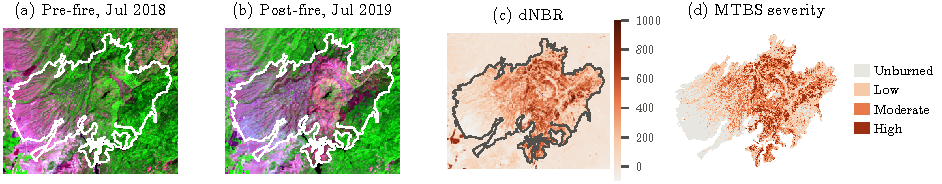
\includegraphics[width=\linewidth]{figs/overview.pdf}
  \caption{The 2018 Camp Fire, showing Landsat surface reflectance before and after the fire as SWIR2, NIR, and red composites from the scenes named in the MTBS record (a, b), the dNBR computed from the two scenes (c), and the MTBS severity map produced by an analyst who chose dNBR thresholds for this fire (d). The white or gray line marks the MTBS fire perimeter, inside which pixels carry labels, and a method receives (a) and (b) as input and predicts (d).}
  \label{fig:overview}
\end{figure}

\section{Problem Formulation}
\label{sec:problem}

For a fire $f$, let $\mathbf{x}^{\text{pre}}_f, \mathbf{x}^{\text{post}}_f \in \mathbb{R}^{6 \times H \times W}$ be Landsat surface reflectance in bands 2--7 (blue, green, red, near infrared, shortwave infrared 1 and 2) before and after the fire, let $\Omega_f$ be the set of unmasked pixels inside the MTBS fire perimeter, and let $y_f(i) \in \{0, 1, 2, 3\}$ denote the MTBS severity class of pixel $i \in \Omega_f$, ordered from unburned through low and moderate to high.
The Normalized Burn Ratio of an image is defined as
\begin{equation}
  \mathrm{NBR} = \frac{\rho_{\text{NIR}} - \rho_{\text{SWIR2}}}{\rho_{\text{NIR}} + \rho_{\text{SWIR2}}},
\end{equation}
where $\rho_{\text{NIR}}$ and $\rho_{\text{SWIR2}}$ are surface reflectance in the near-infrared and second shortwave-infrared bands (OLI bands 5 and 7), and the differenced index $\mathrm{dNBR}_f = 1000\,(\mathrm{NBR}^{\text{pre}}_f - \mathrm{NBR}^{\text{post}}_f)$ is scaled by 1000 following MTBS and \citet{key2006landscape}.
MTBS labels are produced approximately by thresholding this index,
\begin{equation}
  y_f(i) \approx q\big(\mathrm{dNBR}_f(i);\, \boldsymbol{\tau}_f\big), \qquad q(v; \boldsymbol{\tau}) = \sum_{k=1}^{3} \mathbb{1}[v \geq \tau_k],
  \label{eq:mtbs}
\end{equation}
where $\boldsymbol{\tau}_f = (\tau_{f,1}, \tau_{f,2}, \tau_{f,3})$ are the thresholds chosen by the analyst for fire $f$, and the approximation reflects both manual edits and differences between the reflectance processing used here and that of MTBS.

Given a set of labeled training fires $\mathcal{F}_{\text{train}}$, the task is to predict $y_{f^*}$ for a fire $f^* \notin \mathcal{F}_{\text{train}}$ from $\mathbf{x}^{\text{pre}}_{f^*}$ and $\mathbf{x}^{\text{post}}_{f^*}$ alone.
\Cref{eq:mtbs} suggests two strategies for this task, one that estimates thresholds that transfer across fires and another that learns a mapping from reflectance to severity independent of $\boldsymbol{\tau}_{f^*}$.
A predictor with access to $\boldsymbol{\tau}_{f^*}$ would reproduce the analyst's rule up to manual edits, and such a predictor serves below as an oracle that bounds what better calibration could achieve.

\section{Data}
\label{sec:data}

\subsection{Fire Selection}
The dataset contains every wildfire in the MTBS perimeter database that (i) started in California or Oregon in 2018, 2020, or 2021, (ii) burned at least 60{,}000 acres, (iii) was mapped with an extended assessment, in which the post-fire scene is acquired in the growing season after the fire, and (iv) used Landsat 8 or 9 for both scenes.
These criteria yield \mFires{} fires (\cref{tab:fires} in \cref{app:fires}) that together cover \mAcresM{} million acres and span Sierra Nevada mixed conifer, the Klamath Mountains, the western Oregon Cascades, the Coast Ranges, and southern California chaparral, with between \aPxMin{} and \aPxMax{} million labeled pixels per fire.

\subsection{Imagery}
The pre-fire and post-fire scenes identified in each MTBS record are read from the Landsat Collection~2 Level-2 archive \citep{usgs2026landsatc2} hosted on Microsoft Planetary Computer \citep{planetarycomputer}, and for the \mSubstituted{} fires whose exact post-fire scene is missing from the archive, the closest Landsat 9 scene of the same path and row, acquired 8 days later, is used in its place.
Digital numbers are converted to surface reflectance with the Collection~2 scale factor and offset ($\rho = 2.75 \times 10^{-5}\,\mathrm{DN} - 0.2$), each band is warped with bilinear resampling onto the 30\,m Albers grid of the MTBS severity mosaic so that the labels remain on their native grid, and pixels that the Level-2 quality band flags as fill, cloud, dilated cloud, cirrus, cloud shadow, or snow in either scene are masked.
To check alignment, each fire's analyst thresholds are applied to the dNBR computed here and the result is compared with the MTBS map under one-pixel shifts.
For \aAlignShifted{} of the \mFires{} fires (\aAlignShiftedEighteen{} of the \aAlignNEighteen{} fires from 2018 and \aAlignShiftedTwentyOne{} from 2021), agreement is highest at a one-pixel shift, by \aAlignGainMin{} to \aAlignGainMax{} percentage points, and because this offset is left uncorrected it affects every method equally.

\subsection{Labels}
Labels come from the MTBS thematic burn severity mosaics for 2018, 2020, and 2021 \citep{mtbs2024mosaics}, restricted to each fire's perimeter so that neighboring fires in the mosaic are excluded.
Of the six MTBS classes, unburned to low and increased greenness are merged into a single \emph{unburned} class, low, moderate, and high are kept, and the non-processing mask is ignored.
The resulting \mPixelsM{} million labeled pixels are \mShareUnburned\% unburned, \mShareLow\% low, \mShareModerate\% moderate, and \mShareHigh\% high, and the share of high severity ranges from \aHighShareMin\% to \aHighShareMax\% across fires.

\begin{figure}[t]
  \centering
  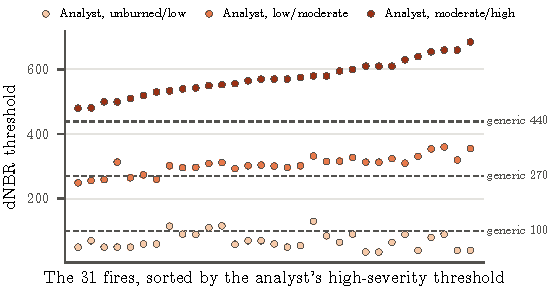
\includegraphics[width=0.78\linewidth]{figs/thresholds.pdf}
  \caption{MTBS analyst dNBR thresholds for the \mFires{} fires, with one column per fire sorted by its moderate/high threshold and dashed lines marking the generic thresholds of 100, 270, and 440.}
  \label{fig:thresholds}
\end{figure}

\subsection{Analyst Thresholds}
Each MTBS record stores the analyst's three dNBR thresholds, and across the \mFires{} fires the unburned/low threshold ranges from \mLowMin{} to \mLowMax, the low/moderate threshold from \mModMin{} to \mModMax, and the moderate/high threshold from \mHighMin{} to \mHighMax{} (\cref{fig:thresholds}).
The generic values of 100, 270, and 440 follow the class edges of \citet{key2006landscape}, whose scheme treats 440--660 as a moderate-high class and reserves the high class for values above 660.

\subsection{Cross-Validation by Fire}
Three pairs of fires in the dataset overlap, as the 2020 North Complex burned into the scar of the 2018 Camp Fire, the 2021 McFarland Fire into the 2020 August Complex, and the 2021 Bootleg Fire into the 2018 Watson Creek Fire.
Fires that share more than 1\% of the smaller fire's area are placed in the same group, and a greedy procedure assigns the groups to five folds while balancing burned area, so that each fold contains \aFoldFiresMin{} to \aFoldFiresMax{} fires and \aFoldAcresMin{} to \aFoldAcresMax{} million acres.
Every method is trained on four of these folds and evaluated on the remaining fold, which by construction contains no fire that overlaps a training fire.

\section{Methods}
\label{sec:methods}

\paragraph{Spectral indices.}
Two relativized indices complement dNBR, namely the relativized dNBR of \citet{miller2007rdnbr} and the relativized burn ratio of \citet{parks2014rbr}, both scaled by 1000,
\begin{equation}
  \mathrm{RdNBR} = \frac{\mathrm{dNBR}}{\sqrt{\max\big(|\mathrm{NBR}^{\text{pre}}|,\, 0.001\big)}}, \qquad
  \mathrm{RBR} = \frac{\mathrm{dNBR}}{\mathrm{NBR}^{\text{pre}} + 1.001}.
\end{equation}
Both indices divide dNBR by a function of pre-fire NBR in order to reduce the dependence of dNBR on pre-fire biomass, and the floor of 0.001 in the RdNBR denominator and the offset of 1.001 in the RBR denominator prevent division by values near zero.

\paragraph{Index thresholding.}
Each threshold classifier applies $q(\cdot; \boldsymbol{\tau})$ from \cref{eq:mtbs} to a single index, and the generic classifier does so for dNBR with $\boldsymbol{\tau} = (100, 270, 440)$.
The learned classifier instead uses the thresholds that maximize mean mIoU over the training fires,
\begin{equation}
  \hat{\boldsymbol{\tau}} = \arg\max_{\boldsymbol{\tau}} \frac{1}{|\mathcal{F}_{\text{train}}|} \sum_{f \in \mathcal{F}_{\text{train}}} \mathrm{mIoU}_f\big(q(\mathrm{index}_f; \boldsymbol{\tau})\big),
\end{equation}
which are found by coordinate search over integer thresholds with step sizes of 64, 16, 4, and 1, using per-fire histograms of the index by class, and weighting every fire equally in this objective prevents the largest fires from determining the thresholds.
The oracle applies dNBR with the test fire's own analyst thresholds $\boldsymbol{\tau}_{f^*}$, and because it draws on information from the test fire, it is reported separately as an upper reference for what per-fire calibration could achieve.

\paragraph{Gaussian smoothing and multi-Otsu.}
This unsupervised baseline smooths dNBR with a Gaussian filter ($\sigma = 1.5$ pixels) and splits the smoothed values inside each fire's perimeter into four classes by multi-level Otsu thresholding \citep{otsu1979threshold}, so that it requires neither labels nor training fires.

\paragraph{Per-pixel gradient boosting.}
A histogram-based gradient-boosting classifier \citep{ke2017lightgbm, pedregosa2011sklearn} with 300 iterations, 63 leaves per tree, and class weights inversely proportional to class frequency is trained on 60{,}000 labeled pixels sampled uniformly from each training fire.
Each pixel is described by 17 features, the 12 reflectance values together with $\mathrm{NBR}^{\text{pre}}$, $\mathrm{NBR}^{\text{post}}$, dNBR, RdNBR, and RBR, and because the classifier sees each pixel in isolation, it provides a reference point that uses the full spectrum without spatial context.

\paragraph{U-Net.}
The U-Net \citep{ronneberger2015unet} has four encoder stages with 32, 64, 128, and 256 channels, a 512-channel bottleneck, transposed-convolution upsampling, and skip connections, for 7.8M parameters in total.
Two variants differ only in their inputs, as the first receives the 12 reflectance bands (\emph{12 bands}) and the second adds the five index channels (\emph{12 bands + indices}), with dNBR, RdNBR, and RBR divided by 1000 and RdNBR clipped to $[-5, 5]$.
Each channel is standardized with the mean and standard deviation of valid pixels in the training fires, and masked pixels are set to zero after standardization.
Training draws $256 \times 256$ patches centered on labeled pixels from fires selected with probability proportional to the square root of their number of labeled pixels, applies random horizontal and vertical flips and $90^\circ$ rotations, and minimizes cross-entropy over labeled pixels with class weights proportional to the inverse square root of class frequency in the training fires.
Each model is trained for a fixed 3{,}000 steps with batch size 16, using AdamW \citep{loshchilov2019adamw} with weight decay $10^{-4}$ and a one-cycle learning-rate schedule \citep{smith2019superconvergence} that peaks at $10^{-3}$, and no checkpoint is selected on held-out data.
At test time a $256 \times 256$ sliding window with stride 128 covers each fire, overlapping predictions are combined with a two-dimensional Hann window, and reflection padding ensures that every pixel receives a prediction, with all hyperparameters listed in \cref{app:impl}.

\section{Experimental Setup}
\label{sec:setup}

\paragraph{Metrics.}
For a fire $f$ and class $c$, $\mathrm{IoU}_{f,c} = \mathrm{TP}/(\mathrm{TP} + \mathrm{FP} + \mathrm{FN})$ is computed over the labeled pixels $\Omega_f$, and the fire's mIoU averages $\mathrm{IoU}_{f,c}$ over the classes present in either the label or the prediction, with macro-F1 and pixel accuracy reported alongside it.
Results are aggregated both as the mean over fires, which weights every fire equally, and as the pooled mIoU of the summed confusion matrices, which weights every pixel equally, and the two can differ because the number of labeled pixels per fire varies by a factor of \aPxRatio.

\paragraph{Statistical comparison.}
Two methods $A$ and $B$ are compared by the mean of the per-fire difference $\mathrm{mIoU}_f(A) - \mathrm{mIoU}_f(B)$, with a 95\% confidence interval from 10{,}000 bootstrap resamples of fires \citep{efron1993bootstrap}, so that whole fires serve as the unit of generalization in the same way that a new fire would.

\paragraph{Implementation.}
All experiments run on a single Apple M5 Pro laptop with 64\,GB of memory, where index thresholding and gradient boosting finish within minutes on the CPU and each U-Net fold trains in about \aMinPerFold{} minutes on the integrated GPU (\aSecPerStep{} seconds per step) with PyTorch \citep{paszke2019pytorch}.

\section{Results}
\label{sec:results}

\begin{table}[t]
\centering
\small
\setlength{\tabcolsep}{3.5pt}
\begin{tabular}{lcccccccc}
\toprule
 & \multicolumn{4}{c}{Mean over fires / pooled} & \multicolumn{4}{c}{IoU per class} \\
\cmidrule(lr){2-5}\cmidrule(lr){6-9}
Method & mIoU & F1 & Acc. & Pooled & U & L & M & H \\
\midrule
Gaussian + multi-Otsu & 0.456\,{\scriptsize$\pm$0.102} & 0.611 & 0.612 & 0.464 & 0.441 & 0.389 & 0.402 & 0.592 \\
dNBR, generic thresholds & 0.564\,{\scriptsize$\pm$0.069} & 0.708 & 0.718 & 0.588 & 0.660 & 0.609 & 0.385 & 0.599 \\
dNBR, learned thresholds & 0.684\,{\scriptsize$\pm$0.058} & 0.808 & 0.820 & 0.709 & 0.662 & \textbf{0.700} & 0.633 & 0.743 \\
RdNBR, learned thresholds & 0.547\,{\scriptsize$\pm$0.122} & 0.693 & 0.700 & 0.564 & 0.571 & 0.552 & 0.475 & 0.588 \\
RBR, learned thresholds & 0.662\,{\scriptsize$\pm$0.060} & 0.793 & 0.802 & 0.683 & 0.644 & 0.675 & 0.608 & 0.722 \\
Per-pixel gradient boosting & 0.678\,{\scriptsize$\pm$0.060} & 0.804 & 0.814 & 0.705 & 0.655 & 0.676 & 0.639 & 0.742 \\
U-Net, 12 bands & 0.684\,{\scriptsize$\pm$0.058} & 0.809 & 0.819 & 0.708 & \textbf{0.664} & 0.690 & 0.636 & 0.745 \\
U-Net, 12 bands + indices & \textbf{0.686\,{\scriptsize$\pm$0.057}} & \textbf{0.810} & \textbf{0.822} & \textbf{0.711} & 0.664 & 0.695 & \textbf{0.642} & \textbf{0.745} \\
\midrule
Oracle (analyst thresholds) & 0.735\,{\scriptsize$\pm$0.043} & 0.845 & 0.854 & 0.752 & 0.702 & 0.736 & 0.693 & 0.808 \\
\bottomrule
\end{tabular}
\caption{Results on 31 held-out fires (fire-grouped five-fold cross-validation, MTBS labels). mIoU, macro-F1 (F1), and pixel accuracy (Acc.) are averaged over fires ($\pm$ one standard deviation across fires). Pooled is the mIoU of the summed confusion matrices. Per-class IoU is averaged over fires, and U, L, M, and H denote unburned, low, moderate, and high. Bold marks the best non-oracle value. The oracle applies each test fire's own MTBS analyst thresholds and is a reference ceiling.}
\label{tab:main}
\end{table}


\Cref{tab:main} reports every method on all metrics, and \cref{fig:summary} shows mean mIoU with bootstrap confidence intervals over fires.

\begin{figure}[t]
  \centering
  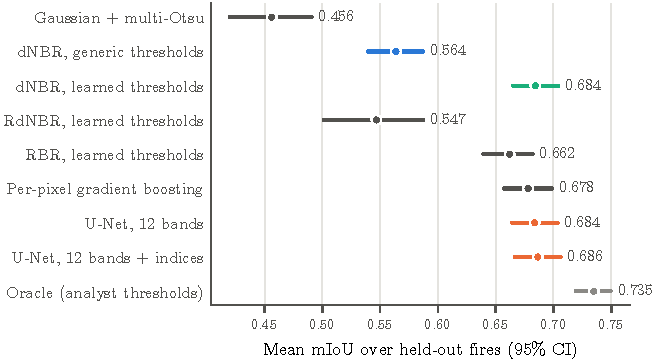
\includegraphics[width=0.66\linewidth]{figs/summary.pdf}
  \caption{Mean mIoU over the \mFires{} held-out fires with 95\% bootstrap confidence intervals obtained by resampling fires.}
  \label{fig:summary}
\end{figure}

\paragraph{Threshold calibration.}
Thresholds learned on the training fires raise mean mIoU from \mdnbrgenericMiou{} to \mdnbrlearnedMiou{} (paired difference \mDiffLearnGen, 95\% CI \mDiffLearnGenLo{} to \mDiffLearnGenHi) and improve \mWinsLearnGen{} of \mFires{} fires.
Across folds, the learned thresholds lie between \mLearnedLowMin{} and \mLearnedLowMax{} for unburned/low, \mLearnedModMin{} and \mLearnedModMax{} for low/moderate, and \mLearnedHighMin{} and \mLearnedHighMax{} for moderate/high (\cref{tab:learned}), which places them close to the analysts' typical values and places the two upper thresholds well above the generic 270 and 440.
The largest per-class change occurs for moderate severity, whose IoU rises from \mdnbrgenericIouModerate{} to \mdnbrlearnedIouModerate{} once the moderate/high threshold moves above the generic value.

\paragraph{Comparison with the U-Net.}
The U-Net trained on 12 bands reaches \munetBandsMiou{} and the variant with index channels reaches \munetIdxMiou, compared with \mdnbrlearnedMiou{} for dNBR with learned thresholds, which corresponds to paired differences of \mDiffBandsLearned{} (95\% CI \mDiffBandsLearnedLo{} to \mDiffBandsLearnedHi) and \mDiffLearned{} (\mDiffLearnedLo{} to \mDiffLearnedHi), with the U-Nets ahead on \mWinsBandsLearned{} and \mWinsLearned{} of \mFires{} fires.
Adding index channels to the U-Net changes mIoU by \mDiffIdxBands{} (\mDiffIdxBandsLo{} to \mDiffIdxBandsHi), and the variant with index channels exceeds per-pixel gradient boosting by \mDiffGbm{} (95\% CI \mDiffGbmLo{} to \mDiffGbmHi), which indicates that spatial context improves on a classifier that lacks it but does not improve on calibrated dNBR.

\paragraph{Relativized indices.}
With learned thresholds, RBR reaches \mrbrlearnedMiou{} and RdNBR reaches \mrdnbrlearnedMiou, and the weaker result for RdNBR reflects its division by the square root of pre-fire NBR, which becomes unstable as pre-fire NBR approaches zero and roughly doubles its standard deviation across fires relative to dNBR (\mrdnbrlearnedMiouSd{} against \mdnbrlearnedMiouSd).
Because MTBS labels are themselves defined by dNBR thresholds (\cref{eq:mtbs}), any other index starts at a disadvantage against these labels regardless of how well it measures severity in the field.

\paragraph{Unsupervised thresholding.}
The Gaussian and multi-Otsu baseline reaches \motsuMiou, the lowest mean and the largest standard deviation across fires (\motsuMiouSd) of any method, because Otsu's method places thresholds that maximize the between-class variance of each fire's smoothed dNBR histogram, and such thresholds need not coincide with severity classes.

\paragraph{Per-fire calibration.}
The oracle reaches \moracleMiou, which is \mDiffOracle{} above learned dNBR (95\% CI \mDiffOracleLo{} to \mDiffOracleHi), and it is better on \mWinsOracle{} of the \mFires{} fires.
When the distance between a fire's analyst thresholds and the learned thresholds of its fold is measured as $\sum_k |\tau_{f,k} - \hat{\tau}_k|$, the oracle's advantage over learned dNBR increases with this distance (Spearman $\rho = \aGapRho$, $p \aGapP$, \cref{fig:calibration}), so the fires on which learned thresholds fall furthest short are those whose analysts departed most from typical thresholds.

\begin{figure}[t]
  \centering
  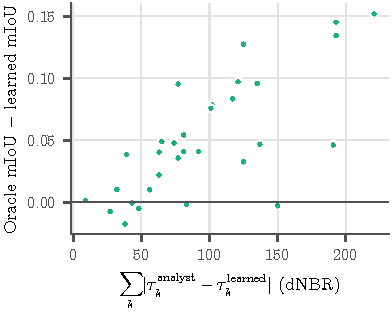
\includegraphics[width=0.46\linewidth]{figs/calibration_gap.pdf}\hfill
  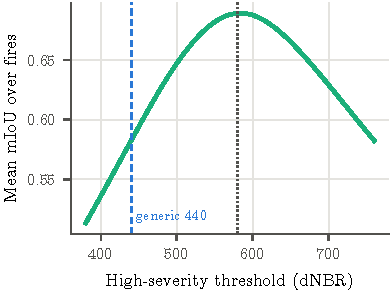
\includegraphics[width=0.46\linewidth]{figs/threshold_sweep.pdf}
  \caption{Oracle advantage over learned dNBR on each fire as a function of the distance between its analyst thresholds and the learned thresholds of its fold (left, Spearman $\rho = \aGapRho$), and mean mIoU over all fires as a function of the moderate/high threshold with the other two thresholds fixed at their mean learned values of \aSweepLow{} and \aSweepMod{} (right). The curve on the right is computed on all fires and therefore describes the dataset as a whole.}
  \label{fig:calibration}
\end{figure}

\paragraph{Per-fire results.}
\Cref{fig:perfire} shows mIoU on every fire, where calibrated dNBR and the U-Net track each other closely and both fall below the oracle on most fires, and \cref{fig:maps} shows the predictions of each method on three held-out fires.

\begin{figure}[t]
  \centering
  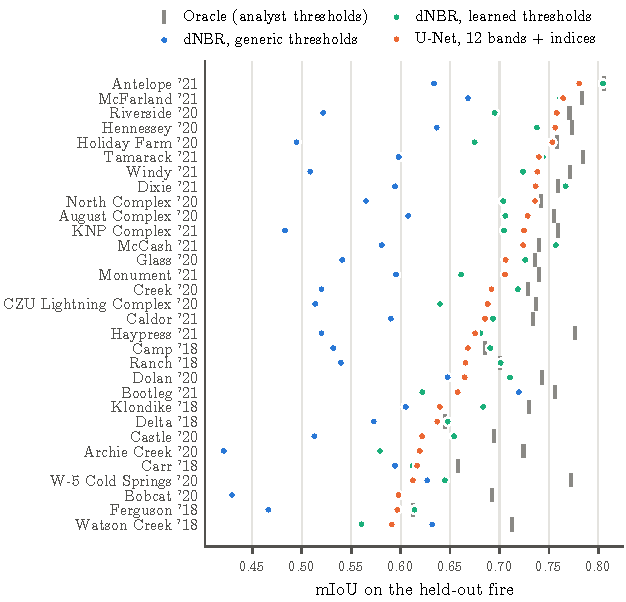
\includegraphics[width=0.62\linewidth]{figs/per_fire.pdf}
  \caption{mIoU of each method on every held-out fire, sorted by U-Net score, with gray ticks marking the oracle.}
  \label{fig:perfire}
\end{figure}

\begin{figure}[t]
  \centering
  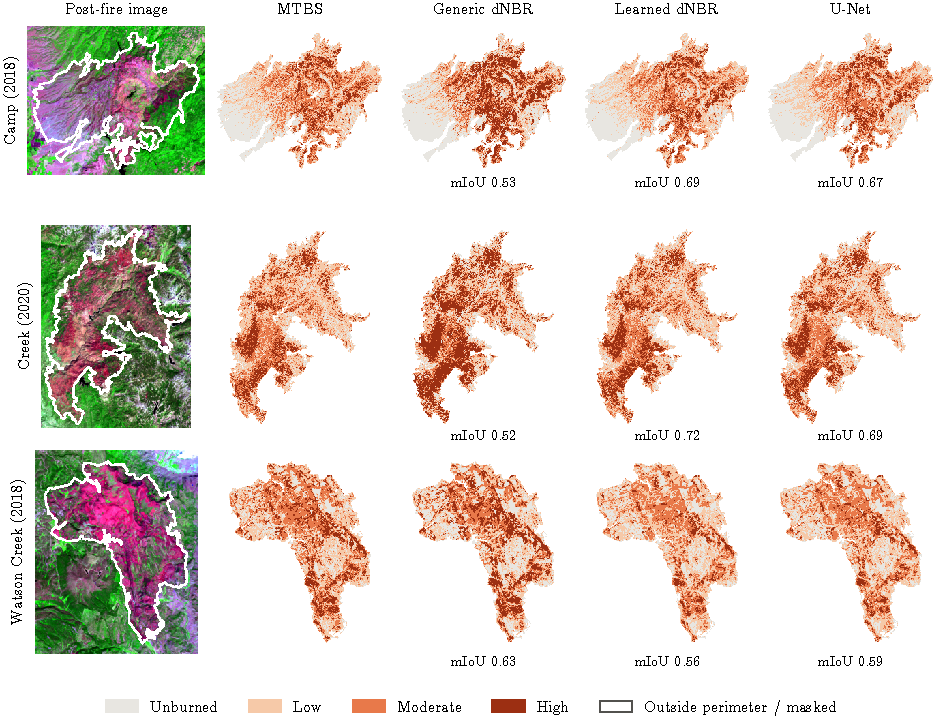
\includegraphics[width=\linewidth]{figs/maps.pdf}
  \caption{Predictions on three held-out fires, namely the Camp Fire, the fire with the median U-Net mIoU (Creek), and the fire with the lowest U-Net mIoU (Watson Creek), each produced by a model trained on the other folds and outlined by the MTBS perimeter in white.}
  \label{fig:maps}
\end{figure}

\section{Analysis}
\label{sec:analysis}

\begin{table}[t]
\centering
\small
\setlength{\tabcolsep}{3.2pt}
\begin{tabular}{lcccccccccccc}
\toprule
 & \multicolumn{3}{c}{Unburned} & \multicolumn{3}{c}{Low} & \multicolumn{3}{c}{Moderate} & \multicolumn{3}{c}{High} \\
\cmidrule(lr){2-4}\cmidrule(lr){5-7}\cmidrule(lr){8-10}\cmidrule(lr){11-13}
Method & P & R & F1 & P & R & F1 & P & R & F1 & P & R & F1 \\
\midrule
dNBR, generic & 80.9 & 86.2 & 83.5 & 87.6 & 67.5 & 76.2 & 65.1 & 48.7 & 55.7 & 63.5 & 99.3 & 77.5 \\
dNBR, learned & 87.3 & 77.8 & 82.3 & 81.0 & 83.9 & 82.4 & 77.4 & 80.5 & 78.9 & 89.1 & 86.7 & 87.9 \\
U-Net (17 ch.) & 82.0 & 84.0 & 83.0 & 82.5 & 81.2 & 81.8 & 78.7 & 79.0 & 78.9 & 88.3 & 88.4 & 88.3 \\
Oracle & 91.9 & 80.2 & 85.7 & 84.3 & 84.6 & 84.4 & 80.8 & 83.1 & 81.9 & 89.2 & 93.0 & 91.0 \\
\bottomrule
\end{tabular}
\caption{\textbf{Generic thresholds lose moderate-severity recall to the high class, and calibration restores it.} Pooled precision (P), recall (R), and F1 (\%) per class over all labeled pixels of the 31 held-out fires.}
\label{tab:perclass}
\end{table}


\paragraph{Bias of generic thresholds.}
Of the errors made by generic dNBR, \aDnbrGenericOverShare\% assign a higher class than MTBS, because the generic moderate/high threshold of 440 lies below every analyst's choice, and as a result high severity has \aDnbrGenericRecHigh\% recall but only \aDnbrGenericPrecHigh\% precision while moderate severity has \aDnbrGenericRecModerate\% recall (\cref{tab:perclass}).
With learned thresholds, moderate recall rises to \aDnbrLearnedRecModerate\% and high-severity precision to \aDnbrLearnedPrecHigh\%, and over-predictions fall to \aDnbrLearnedOverShare\% of errors.

\paragraph{Confusion structure.}
For each of the four methods in \cref{fig:confusion}, at least \aDnbrGenericAdjShare\% of errors confuse classes that are adjacent in the severity order, and no method confuses unburned with high severity at a measurable rate.
The task therefore reduces to placing the boundaries between neighboring classes, which is precisely the role that thresholds play in \cref{eq:mtbs}.

\begin{figure}[t]
  \centering
  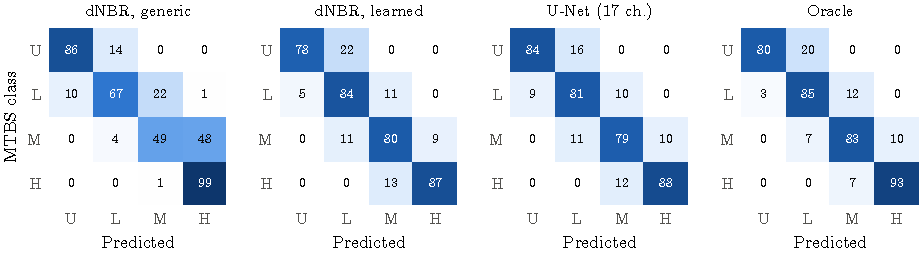
\includegraphics[width=\linewidth]{figs/confusion.pdf}
  \caption{Pooled confusion matrices over all labeled pixels of the \mFires{} held-out fires, normalized by MTBS class in each row and given in percent, where U, L, M, and H denote unburned, low, moderate, and high.}
  \label{fig:confusion}
\end{figure}

\paragraph{Spatial distribution of errors.}
Each labeled pixel is assigned its distance to the nearest labeled pixel of a different MTBS class, and because MTBS maps are spatially fragmented, \aBinShareA\% of labeled pixels lie within 30\,m of another class.
The error rate of learned dNBR is \aDnbrLearnedErrNear\% within 30\,m of a transition and \aDnbrLearnedErrFar\% beyond 240\,m, so that \aDnbrLearnedErrNearShare\% of its errors fall within 30\,m of a transition (\cref{fig:boundary}), and the U-Net follows the same profile with \aUnetBandsIdxErrNear\% and \aUnetBandsIdxErrFar\%.
Near transitions, the median distance between a pixel's dNBR and the nearest analyst threshold is \aThrGapNear{} units, compared with \aThrGapFar{} units beyond 240\,m, so a small difference between the learned and the analyst's thresholds is enough to change the class of these pixels, and the spatial context available to the U-Net does not reduce these errors.

\begin{figure}[t]
  \centering
  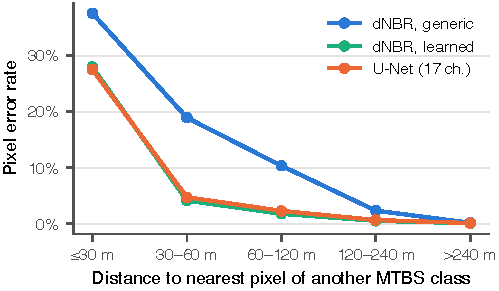
\includegraphics[width=0.56\linewidth]{figs/boundary.pdf}
  \caption{Pixel error rate as a function of distance to the nearest labeled pixel of another class, with the curves for learned dNBR and the U-Net nearly overlapping and \aBinShareA\% of labeled pixels falling in the first bin.}
  \label{fig:boundary}
\end{figure}

\paragraph{Sensitivity to the moderate/high threshold.}
When the unburned/low and low/moderate thresholds are fixed at \aSweepLow{} and \aSweepMod, mean mIoU over all fires peaks at \aSweepBestMiou{} for a moderate/high threshold of \aSweepBest{} and falls to \aSweepAtGeneric{} at 440 (\cref{fig:calibration}, right), and it stays within 0.01 of its maximum for thresholds between \aSweepFlatLo{} and \aSweepFlatHi, a range that lies well above the generic threshold.

\paragraph{Label construction.}
When analyst maps are unavailable, burn severity labels can be derived by applying the generic thresholds to dNBR, but such labels encode a fixed rule computed from the model's own inputs and depend on preprocessing and scene timing (\cref{tab:labels}).
For the Camp Fire, generic thresholds applied to surface reflectance from the MTBS scenes agree with the MTBS map on \mCampGenericPhys\% of pixels and label \mCampGenericHigh\% of the area as high severity, compared with \mCampMtbsHigh\% in the MTBS map.
A per-scene 2nd--98th percentile stretch of each band reduces agreement to \mCampStretch\%, and Landsat 8 median composites whose post-fire window falls in November and December 2018, within weeks of the fire, reduce it to \mCampCompPhys\% without the stretch and \mCampCompStretch\% with it.

\begin{table}[t]
  \centering
  \small
  \begin{tabular}{llcc}
    \toprule
    Imagery & Pre $\rightarrow$ post acquisition & Surface reflectance & Percentile stretch \\
    \midrule
    MTBS scenes & Jul 2018 $\rightarrow$ Jul 2019 & \mCampGenericPhys & \mCampStretch \\
    Landsat 8 median composites & Aug--Nov 2018 $\rightarrow$ Nov--Dec 2018 & \mCampCompPhys & \mCampCompStretch \\
    \bottomrule
  \end{tabular}
  \caption{Agreement (\%) with the MTBS map of the Camp Fire for labels derived by applying the generic thresholds (100, 270, 440) to dNBR, over labeled pixels inside the MTBS perimeter.}
  \label{tab:labels}
\end{table}

\paragraph{Training stability.}
During training of the 12-band U-Net, the loss of one fold became undefined (NaN) at about step 2{,}600, after which that fold's model predicted every pixel as unburned and reached a mean mIoU of \mBandsFoldFourBefore{} on its fires.
This fold alone was retrained with gradient-norm clipping at \mBandsClip, which yielded \mBandsFoldFourAfter, while the other nine U-Net folds were trained without clipping and are reported unchanged, and the variant with index channels trained stably on every fold.

\section{Related Work}
\label{sec:related}

\paragraph{Spectral indices for burn severity.}
The Normalized Burn Ratio contrasts near-infrared reflectance, which healthy vegetation reflects strongly, with shortwave-infrared reflectance, which increases after fire.
\citet{key2006landscape} defined dNBR together with the Composite Burn Index, a field protocol for calibrating it, and \citet{miller2007rdnbr} proposed RdNBR to reduce the dependence of dNBR on pre-fire vegetation.
\citet{parks2014rbr} later proposed RBR, which corresponded more closely to field measurements across 18 fires than either dNBR or RdNBR, while MTBS \citep{eidenshink2007mtbs} applies analyst-selected dNBR thresholds fire by fire, which makes its maps both the standard reference for burn severity and a direct product of per-fire calibration.

\paragraph{Deep learning for burn severity.}
U-Net \citep{ronneberger2015unet} is widely used for dense prediction in remote sensing, and \citet{hu2023burnseverity} trained several U-Net variants on MTBS labels with Landsat imagery across the contiguous United States, finding that an attention U-Net performed best among the architectures they tested.
The comparison here places a U-Net against calibrated index thresholds under an evaluation that holds out whole fires together with their spatial neighbors, and it adds an oracle that isolates the effect of per-fire calibration.

\paragraph{Thresholding.}
Otsu's method \citep{otsu1979threshold} selects thresholds that maximize the between-class variance of a histogram and therefore requires no labels, whereas learned thresholds require labeled fires but are fitted directly to the severity classes.

\section{Discussion and Limitations}
\label{sec:discussion}

\paragraph{Implications.}
For reproducing MTBS maps on new fires, a dNBR classifier with thresholds learned from previous fires is as accurate as the U-Net evaluated here while requiring no GPU and only three interpretable parameters.
The remaining difference from the analyst is a problem of per-fire calibration, and a model that predicts a fire's thresholds from its vegetation, terrain, and imagery would target that difference directly, with the oracle bounding what such a model could gain in this setting.

\paragraph{Reference labels.}
MTBS maps are derived from dNBR with analyst thresholds and manual edits, so they measure agreement with an analyst and favor dNBR over other indices by construction, and evaluating against field measurements such as the Composite Burn Index would instead test how well each method measures burn severity on the ground.

\paragraph{Scope.}
The fires come from two states and three years, fold assignment is fixed, and the evaluation covers one U-Net architecture trained once per fold with a single training budget, so larger models, longer training, or pretraining on more regions may change the comparison.
For two fires the post-fire scene was acquired 8 days after the scene MTBS used, for \aAlignShifted{} fires the imagery and the MTBS labels are offset by up to one pixel (\cref{sec:data}), and the surface-reflectance processing used here differs from MTBS processing, all of which contribute to the error that remains even for the oracle.

\section{Conclusion}
\label{sec:conclusion}

Automatic burn severity mapping was evaluated against MTBS analyst maps on \mFires{} wildfires, with every fire held out together with its spatial neighbors.
dNBR with thresholds learned on other fires reaches a mean mIoU of \mdnbrlearnedMiou, two U-Net variants reach the same accuracy, and an oracle that applies each fire's own analyst thresholds reaches \moracleMiou, with an advantage that grows with how far a fire's thresholds depart from typical values.
Because nearly all remaining errors confuse adjacent classes at class transitions, the limiting factor for automatic burn severity mapping under this evaluation is fire-specific threshold calibration.

\bibliography{refs}
\bibliographystyle{plainnat}

\clearpage
\appendix

\section{Fires}
\label{app:fires}
\begin{table}[H]
\centering
\scriptsize
\setlength{\tabcolsep}{3pt}
\begin{tabular}{lcccccccc}
\toprule
Fire & Year & Fold & Acres (k) & Px (M) & U / L / M / H (\%) & Analyst $\tau$ & Pre-fire scene & Post-fire scene \\
\midrule
August Complex & 2020 & 0 & 1068 & 4.80 & 17 / 29 / 27 / 27 & 110 / 309 / 550 & LC08 2020-07-15 & LC08 2021-07-18 \\
McFarland & 2021 & 0 & 121 & 0.55 & 12 / 40 / 29 / 20 & 89 / 297 / 543 & LC08 2021-07-18 & LC08 2022-07-21 \\
Windy & 2021 & 0 & 98 & 0.44 & 6 / 33 / 33 / 28 & 35 / 313 / 610 & LC08 2021-06-11 & LC08 2022-06-14 \\
CZU Lightning & 2020 & 0 & 86 & 0.38 & 9 / 31 / 26 / 34 & 80 / 354 / 655 & LC08 2020-07-24 & LC08 2021-07-11 \\
Glass & 2020 & 0 & 68 & 0.30 & 15 / 31 / 31 / 23 & 65 / 316 / 595 & LC08 2020-07-15 & LC08 2021-07-18 \\
Dixie$^\dagger$ & 2021 & 1 & 980 & 4.37 & 13 / 32 / 30 / 25 & 70 / 304 / 570 & LC08 2020-07-08 & LC09 2022-07-22 \\
Castle & 2020 & 1 & 174 & 0.78 & 15 / 39 / 33 / 13 & 90 / 310 / 630 & LC08 2020-08-04 & LC08 2021-08-07 \\
Archie Creek & 2020 & 1 & 132 & 0.59 & 3 / 28 / 29 / 39 & 40 / 355 / 685 & LC08 2020-07-22 & LC08 2021-07-25 \\
KNP Complex & 2021 & 1 & 90 & 0.40 & 10 / 43 / 33 / 14 & 35 / 313 / 610 & LC08 2021-06-11 & LC08 2022-06-14 \\
Bootleg$^\dagger$ & 2021 & 2 & 413 & 1.86 & 25 / 23 / 29 / 24 & 70 / 256 / 481 & LC08 2021-06-25 & LC09 2022-07-22 \\
Carr & 2018 & 2 & 234 & 1.03 & 4 / 26 / 35 / 35 & 50 / 259 / 500 & LC08 2018-07-10 & LC08 2019-07-29 \\
Caldor & 2021 & 2 & 227 & 1.02 & 18 / 27 / 24 / 31 & 116 / 312 / 553 & LC08 2021-08-05 & LC08 2022-07-23 \\
Klondike & 2018 & 2 & 178 & 0.62 & 12 / 36 / 22 / 30 & 50 / 313 / 500 & LC08 2018-07-01 & LC08 2019-07-20 \\
Riverside & 2020 & 2 & 138 & 0.62 & 13 / 30 / 20 / 37 & 40 / 331 / 640 & LC08 2019-07-20 & LC08 2021-07-25 \\
Ferguson & 2018 & 2 & 97 & 0.43 & 12 / 44 / 35 / 9 & 50 / 297 / 570 & LC08 2018-07-05 & LC08 2019-07-08 \\
Tamarack & 2021 & 2 & 70 & 0.31 & 17 / 38 / 33 / 11 & 59 / 293 / 556 & LC08 2020-07-01 & LC08 2022-07-07 \\
Watson Creek & 2018 & 2 & 62 & 0.28 & 14 / 37 / 34 / 16 & 50 / 249 / 480 & LC08 2017-08-17 & LC08 2019-08-07 \\
North Complex & 2020 & 3 & 317 & 1.42 & 5 / 24 / 25 / 47 & 90 / 328 / 600 & LC08 2020-08-09 & LC08 2021-07-11 \\
Hennessey & 2020 & 3 & 314 & 1.41 & 34 / 32 / 24 / 11 & 90 / 296 / 540 & LC08 2020-07-08 & LC08 2021-07-11 \\
Monument & 2021 & 3 & 226 & 1.02 & 20 / 34 / 25 / 21 & 115 / 302 / 534 & LC08 2021-07-18 & LC08 2022-07-21 \\
Holiday Farm & 2020 & 3 & 174 & 0.78 & 10 / 27 / 30 / 33 & 40 / 320 / 660 & LC08 2019-07-20 & LC08 2021-07-25 \\
Camp & 2018 & 3 & 154 & 0.69 & 28 / 36 / 25 / 10 & 60 / 301 / 570 & LC08 2018-07-19 & LC08 2019-07-22 \\
Bobcat & 2020 & 3 & 116 & 0.52 & 15 / 41 / 33 / 11 & 130 / 332 / 580 & LC08 2020-07-03 & LC08 2021-07-06 \\
W-5 Cold Springs & 2020 & 3 & 84 & 0.37 & 19 / 62 / 17 / 2 & 60 / 274 / 520 & LC08 2020-08-02 & LC08 2021-08-05 \\
Ranch & 2018 & 4 & 427 & 1.92 & 14 / 36 / 33 / 17 & 55 / 302 / 575 & LC08 2017-07-23 & LC08 2019-08-14 \\
Creek & 2020 & 4 & 382 & 1.71 & 10 / 43 / 30 / 16 & 65 / 324 / 610 & LC08 2020-08-27 & LC08 2021-08-30 \\
Haypress & 2021 & 4 & 204 & 0.86 & 16 / 38 / 25 / 21 & 90 / 360 / 660 & LC08 2020-07-15 & LC08 2022-07-21 \\
Antelope & 2021 & 4 & 142 & 0.64 & 26 / 30 / 22 / 22 & 85 / 315 / 580 & LC08 2021-07-18 & LC08 2022-07-21 \\
Dolan & 2020 & 4 & 124 & 0.56 & 10 / 23 / 33 / 34 & 60 / 260 / 530 & LC08 2020-04-28 & LC08 2021-05-01 \\
McCash & 2021 & 4 & 96 & 0.43 & 15 / 37 / 31 / 18 & 70 / 302 / 565 & LC08 2021-07-18 & LC09 2022-07-20 \\
Delta & 2018 & 4 & 64 & 0.29 & 4 / 25 / 28 / 43 & 50 / 265 / 510 & LC08 2018-07-10 & LC08 2019-07-29 \\
\bottomrule
\end{tabular}
\caption{\textbf{The 31 fires.} Px is the number of labeled pixels inside the MTBS perimeter after masking. U, L, M, and H give the share of labeled pixels in each class. Analyst $\tau$ lists the MTBS dNBR thresholds (unburned/low, low/moderate, moderate/high). Scenes are Landsat Collection~2 Level-2 (sensor, acquisition date). $^\dagger$The archive does not contain the exact MTBS post-fire scene, and the closest Landsat 9 scene of the same path and row, acquired 8 days later, replaces it.}
\label{tab:fires}
\end{table}


\section{Implementation Details}
\label{app:impl}

\begin{table}[H]
  \centering
  \small
  \begin{tabular}{ll}
    \toprule
    Setting & Value \\
    \midrule
    \multicolumn{2}{l}{\emph{U-Net}} \\
    Encoder channels & 32, 64, 128, 256, bottleneck 512 \\
    Parameters & 7.8M \\
    Input channels & 12 (bands) or 17 (bands + indices) \\
    Patch size, batch size & $256 \times 256$, 16 \\
    Training steps & 3{,}000, fixed, no early stopping \\
    Optimizer & AdamW, weight decay $10^{-4}$ \\
    Learning rate & one-cycle, peak $10^{-3}$, 5\% warm-up \\
    Class weights & $\propto$ (class frequency)$^{-1/2}$, training fires \\
    Augmentation & horizontal and vertical flips, $90^\circ$ rotations \\
    Fire sampling & $\propto$ (labeled pixels)$^{1/2}$ \\
    Inference & sliding window, stride 128, Hann weighting, reflection padding \\
    \midrule
    \multicolumn{2}{l}{\emph{Gradient boosting}} \\
    Iterations, leaves & 300, 63 \\
    Learning rate & 0.1 \\
    Class weights & balanced \\
    Training pixels & 60{,}000 per training fire \\
    \midrule
    \multicolumn{2}{l}{\emph{Threshold search}} \\
    Objective & mean mIoU over training fires \\
    Search & coordinate search, steps 64, 16, 4, 1 \\
    \midrule
    \multicolumn{2}{l}{\emph{Gaussian + multi-Otsu}} \\
    Gaussian $\sigma$ & 1.5 pixels \\
    Otsu classes & 4, fit per fire inside the perimeter \\
    \bottomrule
  \end{tabular}
  \caption{Hyperparameters of the U-Net, gradient boosting, threshold search, and Gaussian and multi-Otsu baseline.}
  \label{tab:hparams}
\end{table}

\begin{table}[H]
\centering
\small
\begin{tabular}{cccc}
\toprule
Held-out fold & dNBR & RdNBR & RBR \\
\midrule
0 & 77 / 312 / 579 & 123 / 471 / 816 & 58 / 226 / 390 \\
1 & 82 / 312 / 577 & 122 / 468 / 809 & 59 / 224 / 387 \\
2 & 85 / 319 / 596 & 126 / 474 / 827 & 61 / 229 / 394 \\
3 & 78 / 314 / 587 & 112 / 474 / 828 & 55 / 224 / 393 \\
4 & 81 / 312 / 582 & 123 / 471 / 820 & 59 / 227 / 391 \\
\bottomrule
\end{tabular}
\caption{Thresholds (unburned/low, low/moderate, moderate/high) fit on the four training folds for each held-out fold.}
\label{tab:learned}
\end{table}


\begin{figure}[H]
  \centering
  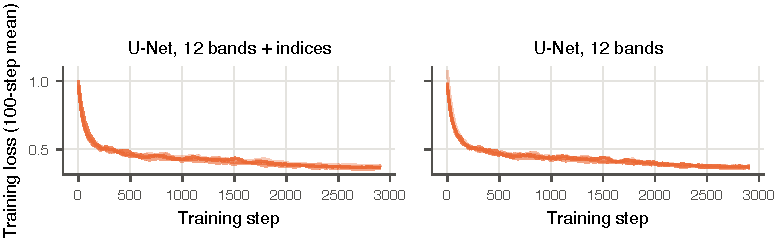
\includegraphics[width=0.85\linewidth]{figs/train.pdf}
  \caption{U-Net training loss per fold as a 100-step moving average, where fold 4 of the 12-band variant shows the run retrained with gradient clipping.}
  \label{fig:train}
\end{figure}

\section{Per-Fire Results}
\begin{table}[H]
\centering
\footnotesize
\setlength{\tabcolsep}{3pt}
\begin{tabular}{lcrcccccc}
\toprule
Fire & Fold & Acres (k) & Otsu & Generic & Learned & GBM & U-Net & Oracle \\
\midrule
August Complex (2020) & 0 & 1068 & 0.448 & 0.608 & 0.706 & 0.741 & 0.728 & 0.755 \\
McFarland (2021) & 0 & 121 & 0.469 & 0.668 & 0.761 & 0.778 & 0.764 & 0.783 \\
Windy (2021) & 0 & 98 & 0.409 & 0.509 & 0.724 & 0.739 & 0.738 & 0.772 \\
CZU Lightning Complex (2020) & 0 & 86 & 0.442 & 0.514 & 0.640 & 0.657 & 0.688 & 0.737 \\
Glass (2020) & 0 & 68 & 0.522 & 0.541 & 0.726 & 0.693 & 0.706 & 0.736 \\
Dixie (2021) & 1 & 980 & 0.455 & 0.594 & 0.767 & 0.731 & 0.736 & 0.759 \\
Castle (2020) & 1 & 174 & 0.486 & 0.513 & 0.654 & 0.633 & 0.622 & 0.694 \\
Archie Creek (2020) & 1 & 132 & 0.370 & 0.421 & 0.579 & 0.579 & 0.619 & 0.724 \\
KNP Complex (2021) & 1 & 90 & 0.475 & 0.483 & 0.705 & 0.713 & 0.725 & 0.759 \\
Bootleg (2021) & 2 & 413 & 0.602 & 0.720 & 0.622 & 0.635 & 0.658 & 0.756 \\
Carr (2018) & 2 & 234 & 0.263 & 0.594 & 0.612 & 0.620 & 0.617 & 0.658 \\
Caldor (2021) & 2 & 227 & 0.484 & 0.590 & 0.693 & 0.719 & 0.685 & 0.734 \\
Klondike (2018) & 2 & 178 & 0.389 & 0.605 & 0.683 & 0.635 & 0.640 & 0.730 \\
Riverside (2020) & 2 & 138 & 0.388 & 0.522 & 0.695 & 0.735 & 0.758 & 0.771 \\
Ferguson (2018) & 2 & 97 & 0.491 & 0.466 & 0.614 & 0.576 & 0.597 & 0.612 \\
Tamarack (2021) & 2 & 70 & 0.566 & 0.598 & 0.744 & 0.713 & 0.740 & 0.785 \\
Watson Creek (2018) & 2 & 62 & 0.454 & 0.632 & 0.560 & 0.539 & 0.591 & 0.712 \\
North Complex (2020) & 3 & 317 & 0.278 & 0.565 & 0.704 & 0.727 & 0.736 & 0.742 \\
Hennessey (2020) & 3 & 314 & 0.586 & 0.636 & 0.738 & 0.764 & 0.757 & 0.773 \\
Monument (2021) & 3 & 226 & 0.503 & 0.595 & 0.661 & 0.723 & 0.706 & 0.740 \\
Holiday Farm (2020) & 3 & 174 & 0.450 & 0.495 & 0.675 & 0.714 & 0.753 & 0.758 \\
Camp (2018) & 3 & 154 & 0.227 & 0.532 & 0.691 & 0.653 & 0.668 & 0.686 \\
Bobcat (2020) & 3 & 116 & 0.510 & 0.429 & 0.597 & 0.614 & 0.598 & 0.692 \\
W-5 Cold Springs (2020) & 3 & 84 & 0.516 & 0.627 & 0.645 & 0.647 & 0.612 & 0.772 \\
Ranch (2018) & 4 & 427 & 0.575 & 0.540 & 0.701 & 0.660 & 0.666 & 0.700 \\
Creek (2020) & 4 & 382 & 0.518 & 0.520 & 0.719 & 0.666 & 0.692 & 0.729 \\
Haypress (2021) & 4 & 204 & 0.535 & 0.520 & 0.681 & 0.648 & 0.675 & 0.776 \\
Antelope (2021) & 4 & 142 & 0.621 & 0.634 & 0.805 & 0.768 & 0.781 & 0.806 \\
Dolan (2020) & 4 & 124 & 0.338 & 0.647 & 0.711 & 0.688 & 0.665 & 0.743 \\
McCash (2021) & 4 & 96 & 0.515 & 0.581 & 0.757 & 0.692 & 0.724 & 0.740 \\
Delta (2018) & 4 & 64 & 0.260 & 0.573 & 0.647 & 0.620 & 0.637 & 0.645 \\
\bottomrule
\end{tabular}
\caption{Per-fire mIoU, where each fire is scored by models trained on the other four folds, Fold gives the cross-validation fold in which the fire was tested, and acres are given in thousands.}
\label{tab:perfire}
\end{table}


\section{Reproducibility}
All code is in the project repository under \texttt{robust/}, where \texttt{fires.py} selects fires and folds from the MTBS perimeter database and \texttt{fetch.py} downloads the Landsat scenes and MTBS labels.
The scripts \texttt{baselines.py} and \texttt{unet.py} train and evaluate every method, and \texttt{report.py} and \texttt{analysis.py} generate every table, figure, and number in the text from the saved predictions.

\end{document}
